% Figure 1: pipeline and the pl02 example (new task set, not seen in the pilot; an illustrative single task).
% Round 10: the Header box reads "names + versions" (H carries the package names, both versions, the tag legend and the
% "follow these lines" sentence); "versions only" described the unrun lockfile-only arm L. Build: pdflatex pipeline.tex (from paper/figures).
% Drawn at the ACL column width (7.7 cm) so that it is included at scale 1; text is 8 pt (\scriptsize at 11 pt).
% Numbers: medians of three runs per arm, new-task study (analysis/round5_table1.json, "figure1_pl02");
% the change line is copied from the frozen 0.4.1 block (notes/tasks2-opus-5-5/pl02.md).
\documentclass[11pt,border=0.5pt]{standalone}
\usepackage{times}
\usepackage[T1]{fontenc}
\usepackage{inconsolata}
\usepackage{tikz}
\usetikzlibrary{positioning,arrows.meta,calc}
\begin{document}
\scriptsize\hyphenpenalty=10000\exhyphenpenalty=10000
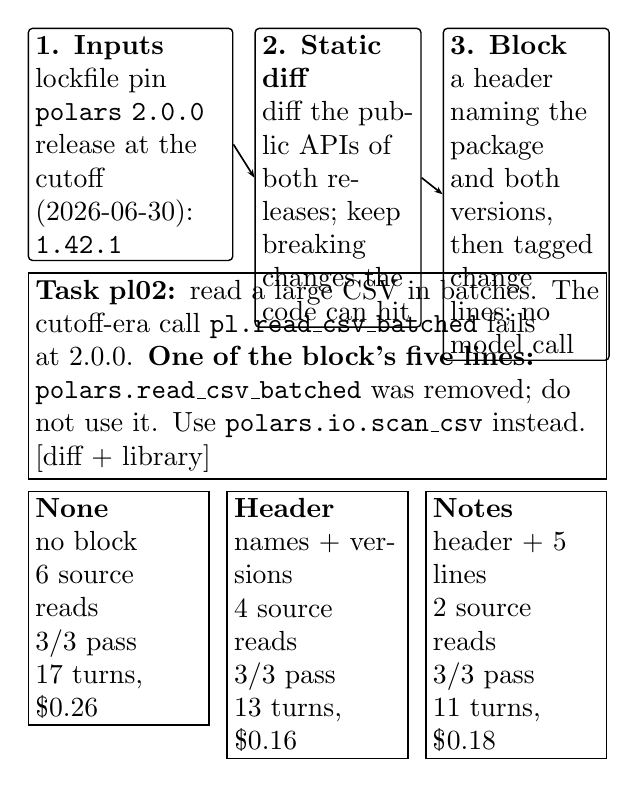
\begin{tikzpicture}[
  box/.style={draw, rounded corners=1.5pt, line width=0.5pt, align=left, inner sep=2.5pt,
              text width=1.93cm, minimum height=2.4cm, anchor=north west},
  wide/.style={draw, line width=0.5pt, align=left, inner sep=2.5pt, anchor=north west},
  arr/.style={-{Stealth[length=3pt]}, line width=0.6pt},
  x=1cm, y=1cm]
  % row 1: pipeline
  \node[box, text width=2.42cm] (in) at (0,0) {\textbf{1. Inputs}\\ lockfile pin\\ \texttt{polars 2.0.0}\\ release at the cutoff\\ (2026-06-30): \texttt{1.42.1}};
  \node[box] (diff) at (2.88,0) {\textbf{2. Static diff}\\ diff the public APIs of both releases; keep breaking changes the code can hit};
  \node[box] (out) at (5.27,0) {\textbf{3. Block}\\ a header naming the package and both versions, then tagged change lines; no model call};
  \draw[arr] (in.east) -- (diff.west);
  \draw[arr] (diff.east) -- (out.west);
  % row 2: the change line
  \node[wide, text width=7.17cm, below=4pt of in.south west, anchor=north west] (note) {\textbf{Task pl02:} read a large CSV in batches. The cutoff-era call \texttt{pl.read\_csv\_batched} fails at 2.0.0. \textbf{One of the block's five lines:} \texttt{polars.read\_csv\_batched} was removed; do not use it. Use \texttt{polars.io.scan\_csv} instead. [diff + library]};
  % row 3: outcomes, medians of three runs each
  \node[wide, text width=2.12cm, minimum height=1.45cm, below=4pt of note.south west, anchor=north west] (a) {\textbf{None}\\ no block\\ 6 source reads\\ 3/3 pass\\ 17 turns, \$0.26};
  \node[wide, text width=2.12cm, minimum height=1.45cm, anchor=north] (h) at ($(note.south)+(0,-4pt)$) {\textbf{Header}\\ names + versions\\ 4 source reads\\ 3/3 pass\\ 13 turns, \$0.16};
  \node[wide, text width=2.12cm, minimum height=1.45cm, below=4pt of note.south east, anchor=north east] (c) {\textbf{Notes}\\ header + 5 lines\\ 2 source reads\\ 3/3 pass\\ 11 turns, \$0.18};
\end{tikzpicture}
\end{document}
